\subsection{Резонансный механизм рождения $e^+e^-$ пар  в полярной шапке магнитара}
Другим процессом, в котором могут иметь место резонансы на виртуальном фотоне и электроне является реакция $\gamma e \to e e^+e^-$, что особенно важно для актуальной в настоящее время  
проблемы генерации электрон-позитронной плазмы в магнитосфере нейтронных звезд и описания особенностей 
радиоизлучения некоторых магнитаров~\cite{Malofeev:2005r, Malofeev:2005,
Duncan:1995,Thompson:1996,Thompson:2002}.  

%Согласно общепринятой модели, для 
%формирования радиоизлучения  в радиопульсаре необходима эффективная генерация 
%электрон-позитронной плазмы в его магнитосфере~\cite{Ruderman:1975}, 
%причем механизмы рождения $e^+e^-$-пар 
%в радиопульсарах хорошо известны (см., например,~\cite{Klepikov:1954,Erber:1966}).  

%
\begin{figure}
\centerline{
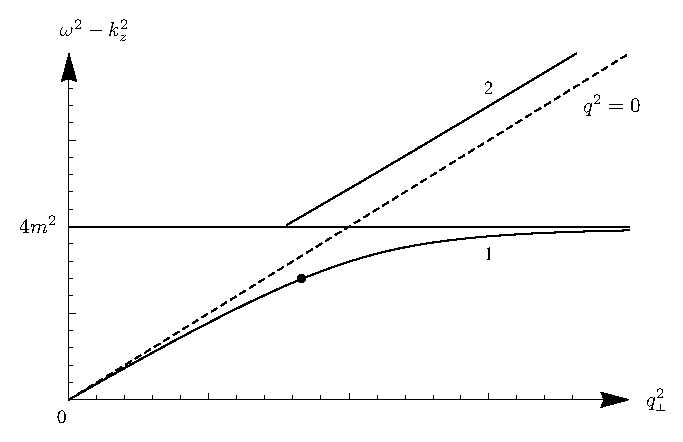
\includegraphics[width=12cm]{fig5_3.eps}}
\caption{ Закон дисперсии фотона в сильном магнитном поле. 
Точкой на дисперсионной кривой 
показано положение фотона, рождающегося в реакции  $e \gamma \to e \gamma$.
 Цифры 1 и 2 обозначают дисперсионные кривые в областях ниже и выше 
порога рождения $e^+e^-$-пар.}
\label{fig:dispersion}
\end{figure}

В модели магнитосферы магнитара рождение $e^+e^-$-пар происходит в два 
этапа~\cite{Beloborodov:2007}. Ускоренная вдоль магнитного поля 
заряженная частица (электрон или позитрон)  
резонансно конвертирует мягкий рентгеновский 
фотон в жесткий, который впоследствии, как предполагается, 
после набора угла между импульсом фотона и направлением 
магнитного поля (так называемый питч-угол), 
должен распадаться на электрон-позитронную пару.  Однако в действительности этого не происходит, так как 
в сильном магнитном поле существенными становятся 
дисперсионные свойства фотона (см. раздел~\ref{Ch:Photon}  и 
рис.~\ref{fig:dispersion}). Такой фотон, рожденный 
в реакции $e\gamma \to e \gamma$ с энергией и импульсом, удовлетворяющими соотношению 
$\omega^2-k_z^2 < 4m^2$ (магнитное поле направлено по оси $z$), в процессе 
распространения 
в магнитном поле будет все время оставаться на дисперсионной ветви 1 и не сможет преодолеть 
зазор между ветвями 1 и 2 с рождением $e^+e^-$-пары, если 
величина магнитного поля $B \gtrsim 0.1 B_e$~\cite{Shabad:1975,ShabUsov:1982,ShabUsov:1985}, 
что заведомо выполняется в магнитарах. 
При достаточно больших $q^2_{\mprp}$ 
такой фотон может лишь перейти на асимптотически больших расстояниях 
в позитроний -- связанное состояние $e^+e^-$-пары. 



В связи с этим представляет интерес рассмотреть альтернативный механизм  рождения 
$e^+e^-$-пар в магнитосфере магнитара. В качестве такого механизма может выступать 
комптоноподобный процесс $\gamma e \to e e^+e^-$, где 
под $e$ в дальнейшем понимается электрон или позитрон. 
Основное преимущество такой реакции по сравнению с принятой 
моделью состоит в том, что рождение пары происходит практически мгновенно в точке взаимодействия 
начальных фотона и электрона 
(в действительности этот масштаб имеет порядок комптоновской длины волны электрона). При таком 
подходе эффект захвата фотона полем становится несущественным. 
Вместе с тем, с помощью 
реакции $\gamma e \to e e^+e^-$ возможно за короткое время заполнить 
ограниченную область 
 достаточно плотной 
$e^+e^-$-плазмой, как, например, 
в процессе гигантской вспышки источника мягких повторяющихся 
гамма всплесков (SGR).

%
\begin{figure}
\centerline{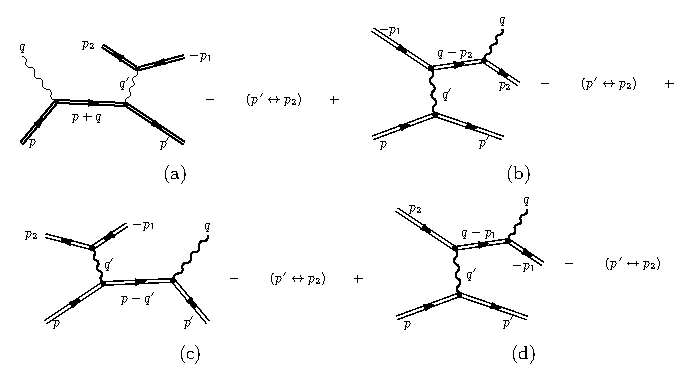
\includegraphics[width=17cm]{fig5_4.eps}}
\caption{Диаграммы Фейнмана для процесса $\gamma + e^{-} \to e^{-} + e^{+}e^{-}$. 
Двойные линии означают, что влияние внешнего поля на начальное и 
конечное состояния учтено точно.}
\label{fig:Diag}
\end{figure}

Процесс рождения электрон-позитронных пар в реакции $\gamma e \to e e^+ e^-$  
описывается восемью диаграммами Фейнмана (см. рис.~\ref{fig:Diag}). Нетрудно 
видеть, что резонанс на виртуальном электроне имеет место только в $s$-канальных 
диаграммах  (рис.~\ref{fig:Diag} $a$ 
и соответствующая диаграмма с перестановкой 
$p^{\, \prime} \leftrightarrow p_2$). Тем  не менее, даже с учетом резонанса 
поставленная 
задача будет иметь достаточно громоздкий вид, поскольку заряженные фермионы могут занимать 
произвольные уровни Ландау. Однако в приложении к магнитарам данную проблему можно 
значительно упростить. Действительно, рассмотрим ситуацию, когда  
электрон, ускоренный в электрическом зазоре полярной шапки 
магнитара, сталкивается с гамма-квантом из равновесной термальной бани, образованной излучением 
рентгеновских фотонов с поверхности нейтронной 
звезды. В такой постановке задачи мы будем иметь следующую иерархию параметров:   
$T^2 \ll m^2 \ll \beta \ll E^2$. Кроме того, электрон, до ускорения 
находившийся на основном 
уровне Ландау $(\ell = 0)$, двигаясь вдоль силовой линии 
магнитного поля, остается все время на основном уровне. 
(Мы рассматриваем небольшую окрестность полярной шапки, где электрическое, 
$\vec {\cal E}$, и магнитное $\vec B$ поля 
коллинеарны и при этом $|\vec {\cal E}| \ll |\vec B|$~\cite{Beloborodov:2007}.) 
 Не нарушая общности будем считать, что  рассеянный
электрон и электрон и позитрон пары также будут находиться на основном уровне Ландау 
 с $\ell^{\, \prime} = n_1 = n_2 = 0$.  Действительно,  как было показано в 
 главе~\ref{Ch:Compton},  
полученный результат для коэффициента поглощения электрона не будет зависеть от состояния конечных частиц, 
а будет определяться только начальными состояниями электрона и фотона.



В окрестности полярной шапки магнитара начальный и рассеянный электрон 
(позитрон), а также 
электрон и позитрон пары будут преимущественно занимать основной уровень Ландау.
С учетом этого замечания  
$S$ -- матричный элемент  процесса $\gamma e \to e e^+ e^-$  может быть записан 
в виде:   
%
\beq
\label{eq:S1}
&&{\cal S}_{\gamma e \to e e^+ e^-} = 
(\ii e)^3 \int d^4 X d^4 Y d^4 Z A_\alpha(X)
\times 
\\[3mm]
\nonumber
&&\times
\big \{ \bar \Psi^{-}_{p',0}(Y) \gamma_{\beta} 
S(X,Y)\gamma^\alpha  \Psi^{-}_{p,0}(X) \bar \Psi^{-}_{p_2,0}(Z) 
\gamma_{\mu} \Psi^{+}_{p_1,0}(Z) -  
\\[3mm]
\nonumber
&&-\bar \Psi^{-}_{p_2,0}(Y) \gamma_{\beta} 
 S(X,Y) \gamma^\alpha \Psi^{-}_{p,0}(X)  
\bar \Psi^{-}_{p',0}(Z) \gamma_{\mu} \Psi^{+}_{p_1,0}(Z) \big \}
G_{\beta \mu} (Z-Y) \, ,
\eeq
входящие в который волновые функции и пропагаторы электронов и фотонов были 
введены в разделах~\ref{Ch:Fermion} и \ref{Ch:Photon} 
соответственно.

                                                      
%После интегрирования~(\ref{eq:S1}) по $d^4X$, $d^4Y$ и $d^4Z$ мы получим 
%%
%\beq
%\label{eq:SV2}                                  
%{\cal S}_{\gamma e \to e e^+ e^-} =   
%\frac{\ii (2\pi)^3 \delta^3 (\ldots) {\cal M}_{\gamma e \to e e^+ e^-}}
%{\sqrt{2\omega V 2 E L_y L_z 2 E^{\, \prime} L_y L_z 2 E_1 L_y L_z 2 E_2 L_y L_z}}\, 
% \, , 
%\eeq
%\noindent где    $\delta^3 (\ldots) \equiv \delta (P_0 - E^{\, \prime}-E_1-E_2) 
%\delta (P_y - p^{\, \prime}_y - p_{1y}-p_{2y}) 
%\delta (P_z - p^{\, \prime}_z -p_{1z}-p_{2z})$, $P_\alpha \equiv (p+q)_\alpha , 
%\,\, \alpha =0,2,3$.
%%
%
%
%Амплитуда процесса $\gamma e\to e e^+e^-$, 
%таким образом, может быть представлена в виде
%%
%\beq
%\nonumber
%&&{\cal M}_{\gamma e\to e e^+e^-} \simeq - \ii \frac{2 \sqrt{2}e^3 m^2}{\pi}  
%\sum \limits_{n=0}^{\infty}
%\; \int \limits^{\infty}_{-\infty} 
%\frac{d q^{\, \prime}_x}{q^{\, \prime 2} - \varkappa^{(2)}(q^{\, \prime})} \; 
%\exp \left [-\frac{\ii (q \varphi q^{\, \prime})}{2e B} \right ] \times
%\\[3mm]
%\label{eq:M11}
%&&\times
%\exp \left [-\frac{\ii(q_x-q^{\, \prime}_x) (p_y+p^{\, \prime}_y)}{2e B} \right ] 
%\exp \left [\frac{\ii q^{\, \prime}_x(p_{1y}-p_{2y})}{2e B} \right ] \times 
%\\[3mm]
%\nonumber
%&&\times 
%\exp \left [- \frac{2q^{\, \prime 2}_{\mprp}+
%q^2_{\mprp}}{4\beta} \right] \; \frac{1}{n!} \left (\frac{(q\Lambda q^{\, \prime})-\ii 
%(q\varphi q^{\, \prime})}
%{2\beta} \right )^n  
% \times 
%\\[3mm]
%\nonumber
%&&\times \frac{(pq^{\, \prime})_{\mprl} [(pq)_{\mprl} + (p^{\, \prime}q)_{\mprl}]}
%{\left (P^2_{\mprl} - m^2 - 2e Bn + \ii P_0 \Gamma_n \right ) 
%\sqrt{q^2_{\mprl}q^{\, \prime 2}_{\mprl} 
%[(pp^{\, \prime})_{\mprl} + m^2]}}_{\bigg |\substack{
%q^{\, \prime \alpha}_{\mprl} = p^{\alpha}_{1 \mprl} + p^{\alpha}_{2 \mprl}\\ 
% q^{\, \prime}_y = p_{1y}+p_{2y}}} -   
%\\[3mm]
%\nonumber
%&&-(p^{\, \prime} \leftrightarrow p_2)\, .
%\eeq

Определяя стандартным путем коэффициент поглощения электрона в 
равновесном фотонном газе, имеющем температуру $T$, 
получим\textcolor{red}{ выразить через $S$}
%
\beq
\label{eq:w1}
W = \int \frac{|{\cal S}_{\gamma e \to e e^+ e^-}|^2}
{\tau}\, 
\frac{Vd^3q}{(2\pi)^3}f_\gamma(\omega)
\frac{L_x L_yd p^{\, \prime}_y  d p^{\, \prime}_z}{(2\pi)^2} \frac{L_x L_yd p_{1y}d p_{1z}}{(2\pi)^2} \frac{L_x L_yd p_{2y}d p_{2z}}{(2\pi)^2}\, . 
\eeq

Как уже отмечалось в разделе~\ref{Ch:Compton}, основной вклад в амплитуду будут 
давать области резонанса, так что 
мы можем использовать дельта-функциональное приближение. Лидирующий вклад от 
уровней Ландау виртуального электрона будет определяться только уровнем с 
$n=1$, вклады высших уровней оказываются подавлены температурой. 
После интегрирования  выражения~(\ref{eq:w1}), с учетом дельта-функционального 
приближения для пропагатора фотона и электрона, получим:
%
\beq
\label{eq:Wfin}
W \simeq  \frac{\alpha\beta  T}{2E^2} \, 
\ln{\left (1- e^{-\frac{\beta}{2ET}} \right )^{-1}} \, .
\eeq


Вероятность рождения $e^+e^-$-пар в единицу времени как функция 
энергии начального  электрона 
представлена на рис.~\ref{fig:prob}. 


%
\begin{figure}[h]
\centerline{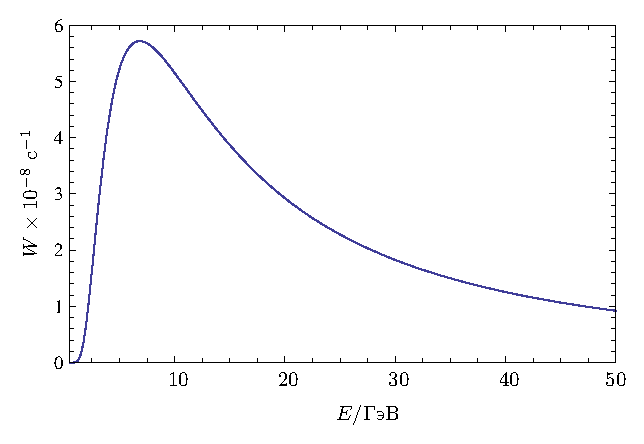
\includegraphics[width=14cm]{fig5_5.eps}}
\caption{Зависимость вероятности рождения электрон-позитронных пар в единицу времени от энергии 
начального электрона  при $B=100B_e$ и $T=1$ кэВ.}
\label{fig:prob}
\end{figure}

Оценивая минимальную длину свободного пробега электрона 
с энергией $E \sim 10^{4} m$ при величинах  
магнитного поля и температуры таких же, как на рис.~\ref{fig:prob}, получим 
$\ell \simeq 57$ см, что 
оказывается много меньше величины зазора $(\sim 100)$ м.  
Вместе с тем изменение числа электронов в потоке за счет рождения пар может быть 
выражено через оптическую толщу $\tau$ следующим образом: 
%
\beq
\label{eq:tau}
N = N_0 \exp{[-\tau]} \simeq N_0 \exp{\left [- \int \limits_0^h d x W \right ]} \, , 
\eeq
\noindent где  $h$ -- ширина электрического зазора, 
$N_0$ -- начальное число электронов в потоке.

Оценивая отношение $N/N_0$ при $h \sim 10^4$ см, $E \sim 10^{7} m$, 
получим $N/N_0 \simeq 0.99$. Таким образом, рассматриваемый 
процесс дает возможность  увеличивать количество $e^+e^-$-плазмы в области 
полярной шапки. Однако детальный количественный анализ 
развития каскада  $e^+e^-$-пар требует 
решения кинетического уравнения, что выходит за рамки настоящего обзора.

Наконец, необходимо сделать еще одно замечание.  Резонансы 
на виртуальных электроне и 
фотоне соответствуют тому факту, что указанные частицы становятся 
реальными. Таким образом,  
рассматриваемый процесс схематично можно представить в виде совокупности трех 
подпроцессов: 
\begin{itemize}
\item
поглощение фотона электроном с рождением электрона на первом уровне Ландау, $e_0+\gamma \to e_1$; 

\item
переход электрона с первого уровня на нулевой с испусканием жесткого $\gamma$-кванта, 
$e_1 \to e_0 + \gamma$;

\item
рождение $e^+e^-$-пары жестким фотоном, $\gamma \to e^+e^-$.

\end{itemize}

Парциальные вклады (branching fractions) последних двух 
реакций приближенно равны 1 и $1/2$ соответсвенно 
(множитель $1/2$ возникает от того, 
что в процессе $\gamma \to e^+e^-$ участвует фотон только одной поляризации из двух возможных). 
Поэтому коэффициент поглощения электрона в  процессе  
$\gamma e \to e e^+e^-$ может быть легко получен из 
вероятности перехода $\gamma + e_0  \to e_1$, как $W = W_{\gamma + e_0 \to e_1}/2$. 
При этом вероятность $W_{\gamma + e_0 \to e_1}$ может быть получена из результатов 
работы~\cite{Latal:1986} и согласуется с~(\ref{eq:Wfin}).
 
 